% プロジェクト学習中間報告書書式テンプレート ver.1.0 (iso-2022-jp)

% 両面印刷する場合は `openany' を削除する
\documentclass[openany,11pt,papersize]{jsbook}

% 報告書提出用スタイルファイル
%\usepackage[final]{funpro}%最終報告書
\usepackage[middle]{funpro}%中間報告書

% 画像ファイル (EPS, EPDF, PNG) を読み込むために
\usepackage[dvipdfmx]{graphicx,color}

% ここから -->
\usepackage{calc,ifthen}
\newcounter{hoge}
\newcommand{\fake}[1]{\whiledo{\thehoge<70}{#1\stepcounter{hoge}}%
  \setcounter{hoge}{0}}
% <-- ここまで 削除してもよい

% 年度の指定
\thisYear{2017}

% プロジェクト名
\jProjectName{ビーコンIotで函館のまちをハックする}

% [簡易版のプロジェクト名]{正式なプロジェクト名}
% 欧文のプロジェクト名が極端に長い(2行を超える)場合は、短い記述を
% 任意引数として渡す。
%\eProjectName[Making Delicious curry]{How to make delicious curry of Hakodate}
\eProjectName{Leverage the Beacon Iot in Hakodate Real Down town for Our Smarter Life}


% <プロジェクト番号>-<グループ名>
\ProjectNumber{8-B}

% グループ名
\jGroupName{Youbeacomm}
\eGroupName{Youbeacomm}

% プロジェクトリーダ
\ProjectLeader{1015253}{橋場保鷹}{Hodaka~Hashiba}

% グループリーダ
\GroupLeader  {1015215}{藤原祐汰}{Yuta~Fujiwara}

% メンバー数
\SumOfMembers{5}
% グループメンバ
\GroupMember  {1}{1015074}{河田歩美}{Ayumi~kawada}
\GroupMember  {2}{1015215}{藤原祐汰}{Yuta~Fujiwara}
\GroupMember  {3}{1015240}{荒田啓太郎}{Keitaro~Arata}
\GroupMember  {4}{1015250}{高橋大輔}{Daisuke~Takahashi}
\GroupMember  {5}{1015253}{橋場保鷹}{Hodaka~Hashiba}


% 指導教員
\jadvisor{松原克弥,藤野雄一,鈴木恵二,奥野拓}
% 複数人数いる場合はカンマ(,)で区切る。カンマの前後に空白は入れない。
\eadvisor{Katsuya~Matsubara,Yuichi~Fujino,Keiji~Suzuki,Taku~Okuno}

% 論文提出日
\jdate{2017年7月21日}
\edate{July~21, 2017}

\begin{document}
%
% 表紙
\maketitle

%前付け
\frontmatter

% 和文概要
\begin{jabstract}
   本プロジェクトは、フィールドを実際に調査してそこから問題点を見つける。そこで見つかった問題点をビーコンを活用して、より函館のまちをよくするサービスの提案・開発を行う。
  実際に函館で行ったフィールドワークの結果、外国人観光客が地元民との会話に苦戦している様子が多く見られた。
  この問題は指差し会話帳が普及することで解決できると考えた。しかし既存の指差し会話帳は、扱いにくいという点がある。
  よってグループBでは、既存の指差し会話帳を改良・発展させ、外国人観光客が日本人とスムーズに会話できるようにできるようなアプリケーションの提案をした。
  しかしこの提案を7月14日に行われた中間報告会で発表したところ、たくさんの課題が見つかった。後期では課題を元にグループで提案を改善しプロトタイプの作成をする。
  そのプロトタイプを用いて実際に外国人観光客に使用してもらい、レビューをいただく予定である。そしてこれを繰り返すことで外国人観光客にあったシステムデザインを行っていく。
%\fake{桜ひなのです}
% 和文キーワード
\begin{jkeyword}
函館, ビーコン, 外国人観光客, 指差し会話帳, システムデザイン
\end{jkeyword}
\bunseki{藤原祐汰}
\end{jabstract}

%英語の概要
\begin{eabstract}
   This project actually examines the field and finds problems from there.
   We make use of beacon to solve the problem found, and we will propose and develop a service that better Hakodate's town.
  As a result of the fieldwork actually carried out in Hakodate, there were many cases where foreign tourists struggled with conversation with locals.
  I thought that this problem could be solved by dissemination of the pointing conversation book. However, existing pointing conversation book has a point that it is difficult to handle. Therefore, in Group B, we improved and developed the existing pointing conversation book, and proposed an application that enables foreign tourists to talk with Japanese smoothly. However, when this proposal was announced at the interim report meeting held on July 14, a lot of subjects were found. In the latter term, we will improve the proposal by the group based on the task and create a prototype. Using that prototype will actually be used by foreign tourists and will be reviewed.
  And by repeating this we will do system design suitable for foreign tourists.
%\fake{you should write your English abstract in one page. }
% 英文キーワード
\begin{ekeyword}
  Hakodate, Beacon, Foreign Tourists, Pointing Conversation Book, System Design
\end{ekeyword}
\bunseki{藤原祐汰}
\end{eabstract}

\tableofcontents% 目次


\mainmatter% 本文のはじまり

\chapter{はじめに}

\section{背景}
\subsection{函館について}
 函館市は、北海道の中にある市の一つで人口はおよそ26万人の都市である。函館市は夜景や歴史的建造物、温泉といった多くの観光地を持っているため日本人だけではなく、多くの外国人観光客が函館を訪れる。
平成28年度における観光入込客数は、上期(4月~9月)は約366万5千人(前年同期に比べ約45万4千人増の114.1%)、下期(10月~3月)は約194万2千人(約20万6千人増の111.9%)、合計約560万7千人(約66万人増の113.3%)となった。
さらに外国人宿泊客数については、台湾や中国だけでなく、近年はタイ、マレーシアなどの東南アジアからの宿泊客が増加し、全体でも約40万5千人(約7千人増、前年比101.9%)と過去最高を更新した[1]。
以上のことから、現在函館には多くの外国人観光客が訪れることがわかる。しかし、外国人が函館を観光する上でさまざまな問題を抱えている。
\bunseki{藤原祐汰}

\subsection{函館の抱える問題}
 毎年多くの外国人観光客が訪れる中での問題点は、地元民がどう他言語に対応するかという問題である。母国語で話をしてくる外国人観光客が、何を伝えたいのか理解するのが難しく、同じ言語で会話するレベルでの意思疎通を図ることは非常に困難である。ここで「指差し会話帳」というものがある。
指差し会話帳とは、自分の伝えたいフレーズが、伝えたい側の言語に訳されており、指をさすだけで会話ができるという本のことである。しかし既存の指差し会話帳にはいくつか扱いにくい点が2つある。
1つ目は、掲載されているフレーズ多いという事である。そのために、自分の伝えたいフレーズがどこに掲載されているのかわからず、本の扱いに慣れるまでは見つけにくいという点である。
2つ目は、掲載されているフレーズがどこの旅行先でも使えるようなフレーズしか掲載していないという事である。
つまりこの本の中にあるフレーズでしか会話することができないため、この本以外の質問は機械翻訳や身振り手振り、文法が誤っている片言で会話するしか方法がないのである。
\bunseki{藤原祐汰}

\subsection{課題の概要}
 以上のように、外国人観光客と函館の地元民の会話を手助けするものが整備されていない
ということが函館の課題である。
\bunseki{藤原祐汰}



\chapter{プロジェクト学習の概要}

\section{本プロジェクトにおける目的}\label{sec:mokuteki}
 本グループでは、外国人観光客と日本人をつなぐコミュニケーション促進サービスを提供することを目指し、
「ビーコンを用いて外国人観光客と日本人の会話をスムーズに行えるよう手助けをすること」を目的とした。
\bunseki{藤原祐汰}

\section{課題の設定}
\ref{sec:mokuteki}~で述べた目的を実現するにあたり、私たちはビーコンを用いての、
スマートフォンアプリケーションを作成することとした。
\bunseki{藤原祐汰}

\section{ビーコンについて}
\subsection{ビーコンの概要}
 ビーコンとは、Bluetoothの電波を発している小さな機器である。
その電波をスマートフォンで受信することで、ビーコンがあることや、ビーコンまでの距離がわかり、
屋内外の区別なく位置に応じたサービスの提供ができるIot機器である。
\bunseki{藤原祐汰}

\subsection{ビーコンを使ったサービスの例}
 Tangerine株式会社では、「店舗内アーティスト動画視聴サービス」を大手CDレンタルチェーン店で行っている。
これは店舗内のビーコンが自分のスマホを検知している間は音楽視聴が可能であるというものである。
このサービスによって、視聴ブースの混雑回避や、来店客が店内を楽しく自分のスマホで気軽に試聴を楽しむことができるようになった。
またtranscosmos株式会社では、「OFFERs」という顧客に合わせたコンテンツを配信・効果測定可能なスマホマーケティングツールのサービスを提供している。
これはプッシュ通知・電子DMで顧客へクーポン・レコメンドを配信するというものである。
\bunseki{藤原祐汰}

\subsection{ビーコンの概要}
 今回はTangerine株式会社、transcosmos株式会社が本プロジェクトの為、ビーコンを函館市内におよそ1000個ほど、設置する役割となっている。
さらに私たちのビーコンに対する理解を深めるため、ビーコンを用いた開発についてのレクチャーを受けた。
\bunseki{藤原祐汰}



\chapter{Youbeacommについて}
\section{Youbeacomについての概要}
 Youbeacommは外国人旅行者と日本人をつなぐコミュニケーション促進サービスとして、お互いに共通の言語がない人々に対し、そのコミュニケーションをソフトウェアによって支援する。
同様の課題への解決策として、「指さし会話帳」という、様々なフレーズや単語が2言語で併記されている書籍が市販されているが、
掲載されている情報量が多いことのデメリットとして、旅行先での各場面ごとに適切な情報を絞り込むことが困難であることがあげられる。
また、紙媒体である以上、同一のコンテンツを重複して掲載することは難しく、利用者の想像と全く異なるジャンルのページに掲載されていることもある。
本提案手法では利用者の現在地や移動経路、時間帯、天候など、コミュニケーションで支援が必要となる状況に至る数多くの要素を「コンテキスト」と呼び、それらの情報を基にしたフレーズや単語の絞り込みや優先度付けを行うことで、
利用者がその時点で正に求めている候補を提案することを目指す。
\bunseki{高橋大輔}
\section{Youbeacommの具体的なシステムの説明}
 本システムへのアクセスは外国人旅行者向けのスマートフォンのアプリとして提供する。アプリはGPS, (設置するビーコンを含む) Bluetooth Low Energy, Wi-Fiなどの情報をバックグラウンドで定期的に取得し、
利用者の起動操作によって、フォアグラウンドとなった時点で、それらの情報をサーバに送信する。サーバはコンテキストを認識し、アプリに対してそれに応じたフレーズを応答することで、フレーズの提案が行われる。
利用者は提案されたフレーズから適切なものを選択し、コミュニケーションの相手に提示したのち、スマートフォンを相手に渡して、
同様に、システムの提案の中から適切な回答を選択してもらう。
提案の中に適切なフレーズがない場合のフォールバックとしては、機械翻訳や観光案内所、電話による通訳サービスなどの案内を行う。
また、適切なフレーズの提案がなかったこと自体については、提案されたフレーズに対して、利用者がフィードバックや追加の提案を行えるようにすることで、フレーズの充実、並びに提案精度の向上を図る。
\bunseki{高橋大輔}




\chapter{中間報告会}

\section{発表形式}
7月14日に行われた中間報告会では, 各グループの行ってきた活動を詳細に伝え, 後期の活動に活
かせるレビューを得ることを目的とした. 発表としては, 全体のポスターを5分程度で発表し, その
後に各グループごとに並列で7分程度の3つの発表を行った. その後は時間の許す限り質疑応答の
時間とした
\bunseki{荒田啓太郎}

\section{レビュー内容}
\subsection{発表方法についての評価と反省}
以下に, 中間発表会で行ったアンケートの「発表技術について」の項目から, 最終成果発表にも
取り入れたいものをまとめた
\begin{itemize}
 \item ポスターの図からは多言語対応しているように見られない.
\end{itemize}
上記は, 口頭での説明でも欠如していた内容であり, スクリプトとポスターの完成度不足が伺える.
一方で, ポスターがわかりやすいとの評価も受けた.
\bunseki{荒田啓太郎}
\subsection{発表内容についての評価と反省}
以下に, 中間発表会で行ったアンケートの「発表技術について」の項目から, 最終成果発表にも
取り入れたいものをまとめた.
\begin{itemize}
 \item 会話のきっかけを生むことはできるが, 会話を成立させるための工夫が必要.
 \item 指さし会話帳の認知度をそのような手段で向上させていくのか.
\end{itemize}
上記より得られた見落としは, 多岐にわたる会話のパターンと, このアプリの認知度である. ユーザ
はこのアプリの使い方を知らない. 他人から突然スマホを見せられて質問を円滑に, そして快く回
答する人は少ないだろう. こういった問題を解決するためにもアプリの流れの明快さの向上や, ア
プリ自体の認知度の向上に努めるべきである. 外国人観光客をターゲットにするならば, アプロー
チはその出入りが激しい場面で行うべきだと感じた. そのため, 最終成果発表までに認知度の向上
方法やUI部分の改善に努めることで, このアプリの価値を高めていきたい。
\bunseki{荒田啓太郎}



\chapter{今後の予定と展望}

\section{今後の予定}
 始めに制作の流れを説明する。提案した案の見直しをして、簡単なプロトタイプを作り、そのあとにアプリケーション開発を進めていく。開発し終えた後、作ったアプリケーションを実際に使用してもらい、そのフィードバックから改善を行っていく。
次にプロセスに沿って詳しい説明する。後期の始めに、前期の中間報告会で提案したアイデアの、発表を聞いていただいた方々から受けたフィードバックを取り入れ、提案の改善を行う。次に、改善した内容を基にシステムを開発する。
制作については、アプリケーションを制作していく。私たちが提案するサービスは外国人を対象としたアプリケーションであるが、函館に観光しに来る外国人がどのスマートフォンを使っているかが想定できないため、AndroidとiOSの両方に対応したアプリケーションを作っていくことを予定している。
アプリケーションの制作は、開発を行う前にメンバー同士の考えに相違点が生じないようプロトタイプを作って、内容を確認し合ってから開発を行おうと思っている。
アプリケーションを作り終ったら、実際に函館市内にいる外国人観光客に使用してもらい、使った感想や改善した方がいい点を聞き、再びアプリケーションの改善を行う。
アプリケーションの改善と実際に使用してもらうことを何度か繰り返し行うことによって、私たちの提案するサービスの完成度を上げていく。
\bunseki{河田歩美}

\section{今後の展望}
 私たちが開発するアプリケーションでは、既存の機械翻訳を利用する。既存の機械翻訳をコンテキストに沿って文章の提供することで、翻訳の精度が上がると予測される。
 間違った翻訳をしてしまうと、相手に間違った内容を伝えてしまい、意図している会話が成り立たない可能性も考えられるので、開発する際にこの点は重要視していきたいと考えている。
\bunseki{河田歩美}



\chapter{前期の振り返りと学び}
\section{振り返り}
\subsection{スケジュール管理}
 スケジュール管理については、プロジェクト開始時に決定した年間スケジュールを元に管理を行った。
前期での活動では、年間スケジュールと概ね一致した活動や成果を出せた為、管理を行えていたといえる。
しかし、問題点としてスケジュール管理者が制作したスケジュールを早い段階から全体に公開していなかった事が挙げられる。
これによって、メンバーの多数が今自分が何をやっているのかについての理解に時間を要してしまった。
後期のプロジェクトでは、これを改善し、スケジュール管理者とメンバーとの意思疎通や、意見交換会を実施することで認識の齟齬を無くすことが重要であるといえる。
\bunseki{橋場保鷹}
\subsection{情報共有}
 私たちは、本プロジェクトが始まった当初、議題に対してプロジェクト全体で発表や共有、意見の交換を行っていた。
しかし、大人数で作業を行う際、アウトプットされる意見が少なかったり、情報伝達が行き届いていなかったりといった問題点があった。
そこで、私たちは3人から4人の小グループを作り、そこで討論を行なうといった手法を用いた。
人数を絞ることで個人が意見を出しやすい環境を作り、議論の効率化を図ったことにより、
より多くの意見をアウトプットさせることが出来た。
よって、私たちが後期のプロジェクト学習を行うに当たって、
小グループでのディスカッションを多く取り入れることが今後も重要になってくると考えられる。
\bunseki{橋場保鷹}

\section{学び}
\subsection{システム設計}
 私たちは、前期のプロジェクトを通してより実践的にどのようにしてシステムを設計するのかを学ぶことが出来た。
プロジェクト内でシステム設計についての考え方や、有用性のレクチャーを行ない、
本学の講義であるソフトウェア設計で学んだ技術を用いて実際に提案したサービスの設計を行った。
実際に自身で考えたサービスにシステムを肉付けしていくといった段階を踏んだ事により、
全体を通してより実践的なシステム開発技術を習得できたといえる。
\bunseki{橋場保鷹}
\subsection{情報をアウトプットする技術}
 私たちは、前期のプロジェクトを通して積極的に情報のアウトプットを行ってきた。
ブレーンストーミングやアイデアソンを通して、メンバー個人が保有している情報や発想を洗い出しを行った。
また、外部企業を招いてのアイデアコンテストや、函館市のものづくり企業紹介の場へ参加し、
自らの提案を積極的に外部へアウトプットした。
これらの経験により、プレゼンテーションを行うスキルや、内部情報を知らない外部の関係者がどのような情報を必要としているのかを知ることができ、
その情報をメンバー間で共有することで全体としてアウトプット技術の向上を図ることが出来た。
\bunseki{橋場保鷹}

% 以降、付録(付属資料)であることを示す
\begin{appendix}

\chapter{中間報告会で使用したグループBのポスター}
\begin{center}
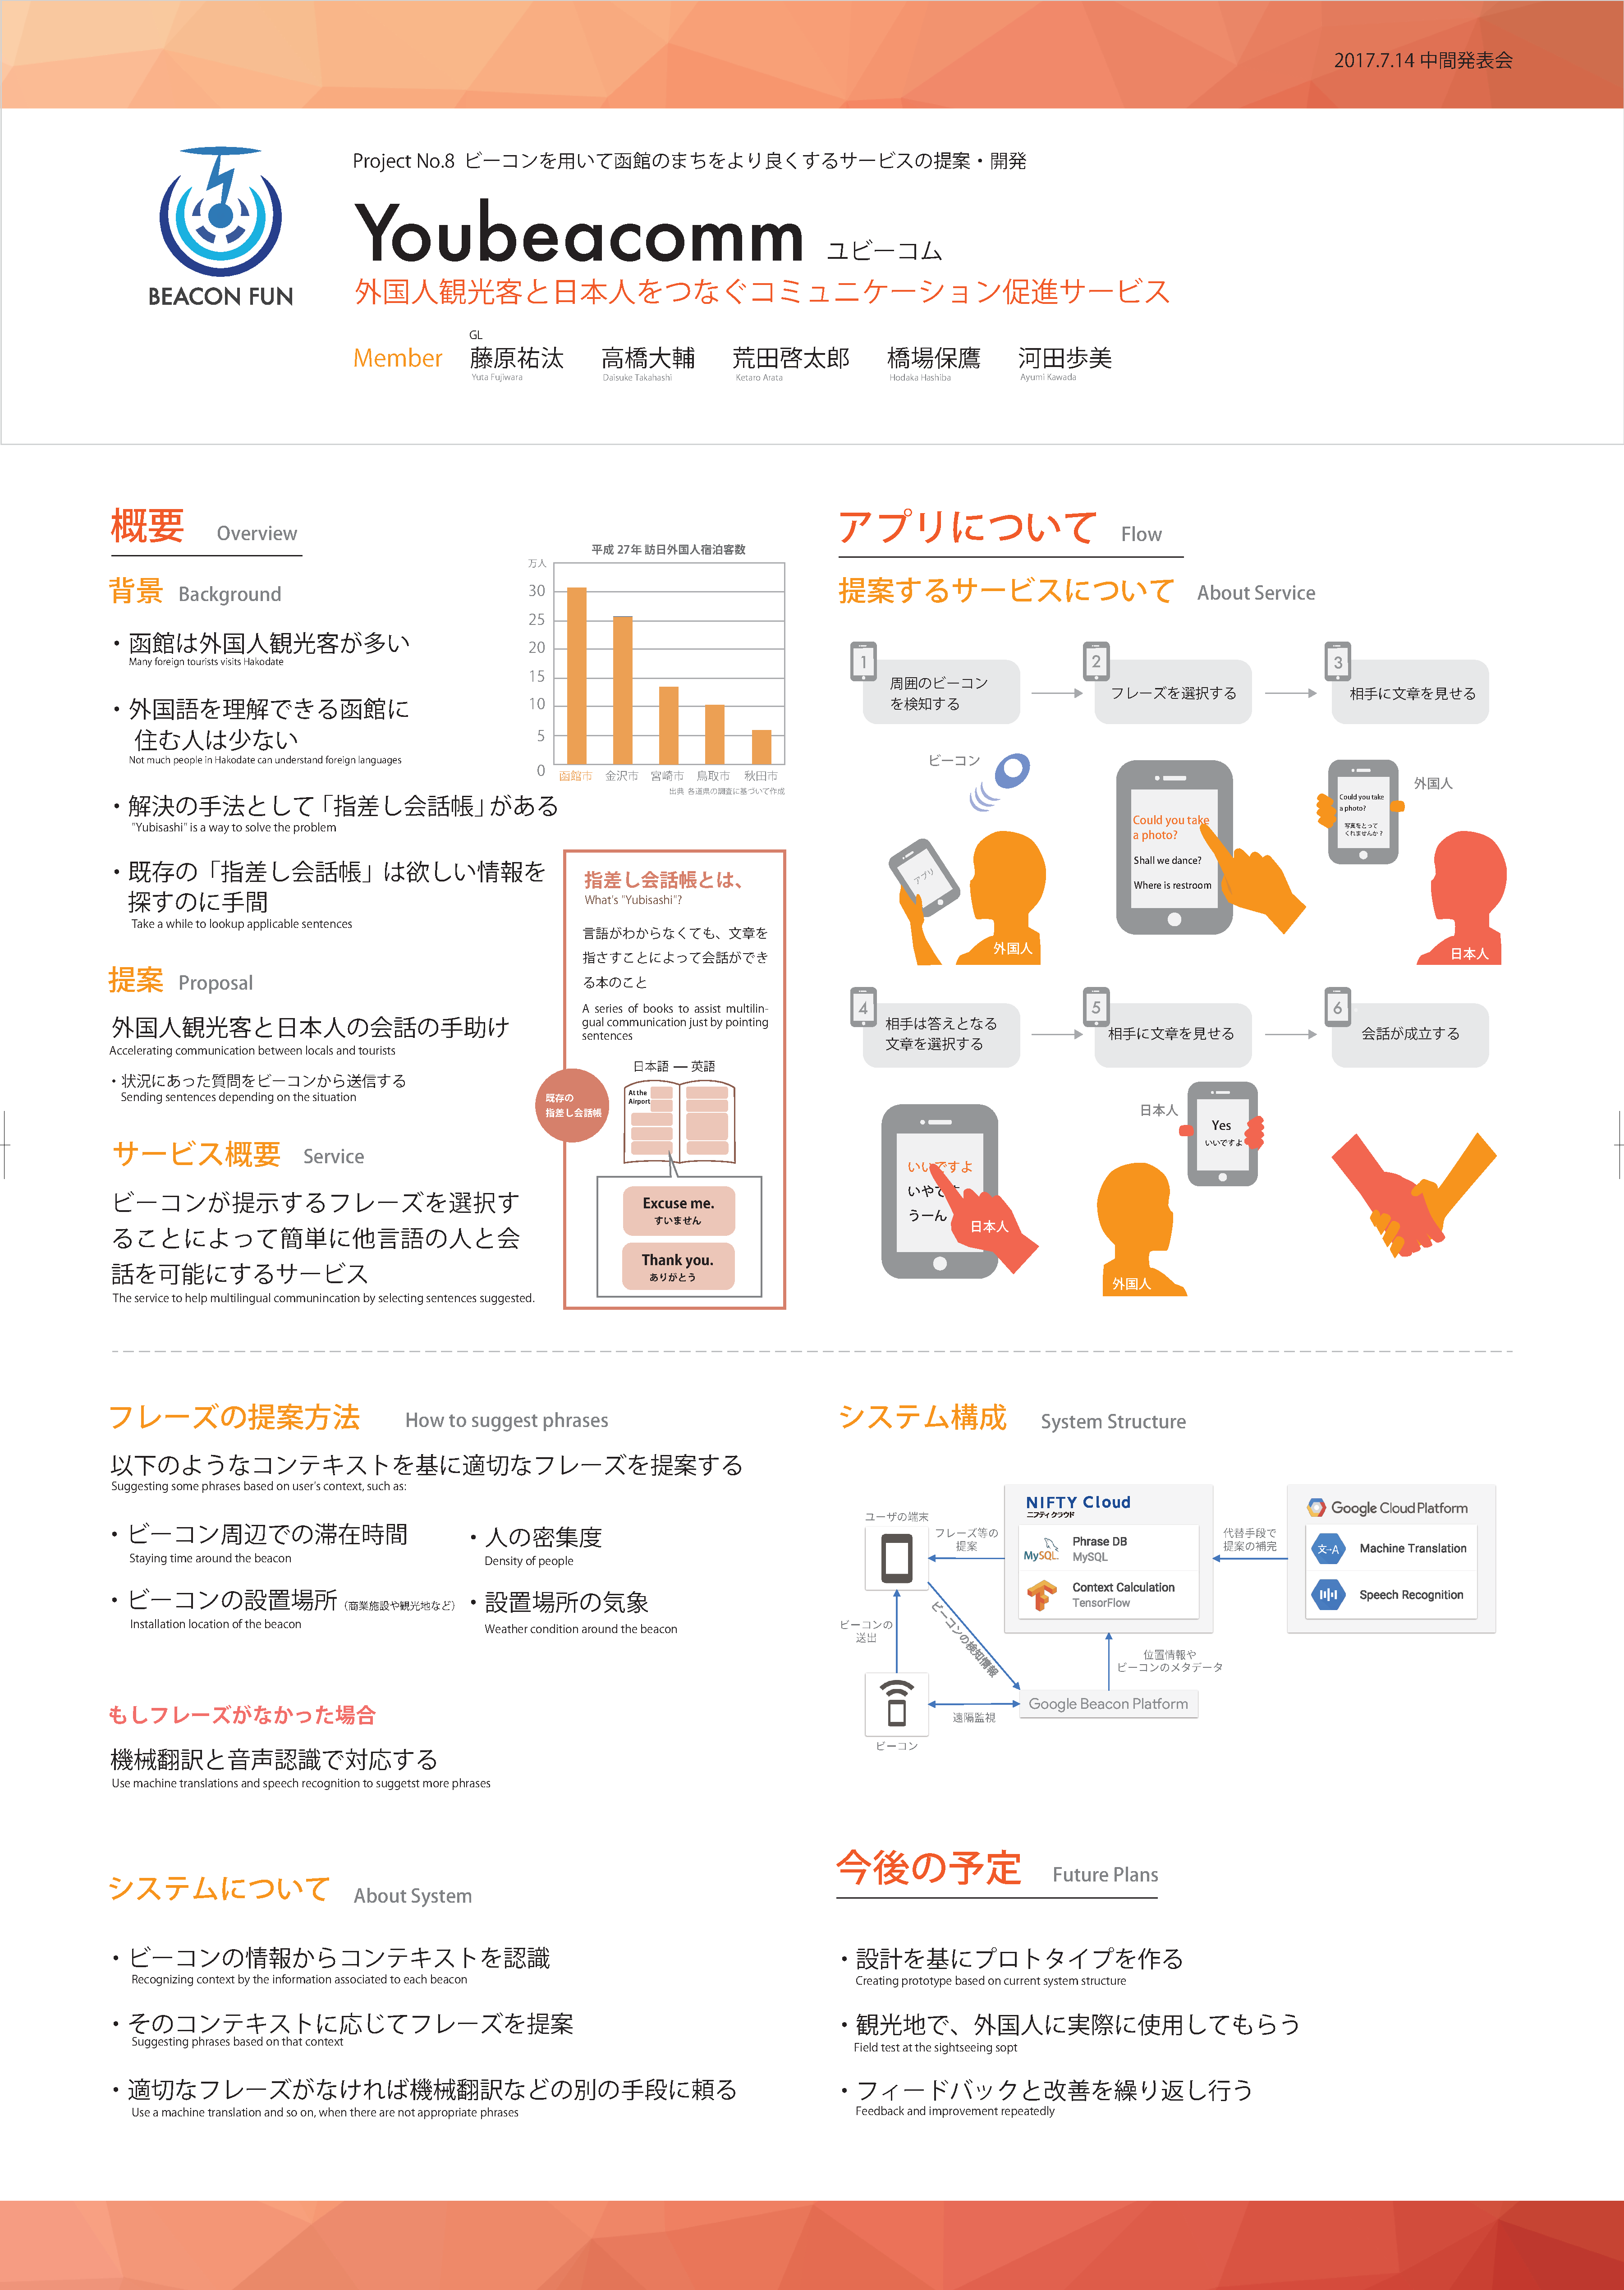
\includegraphics[width=13cm]{gbt.pdf}
\end{center}

\chapter{Youbeacommの画面遷移図}
\begin{center}
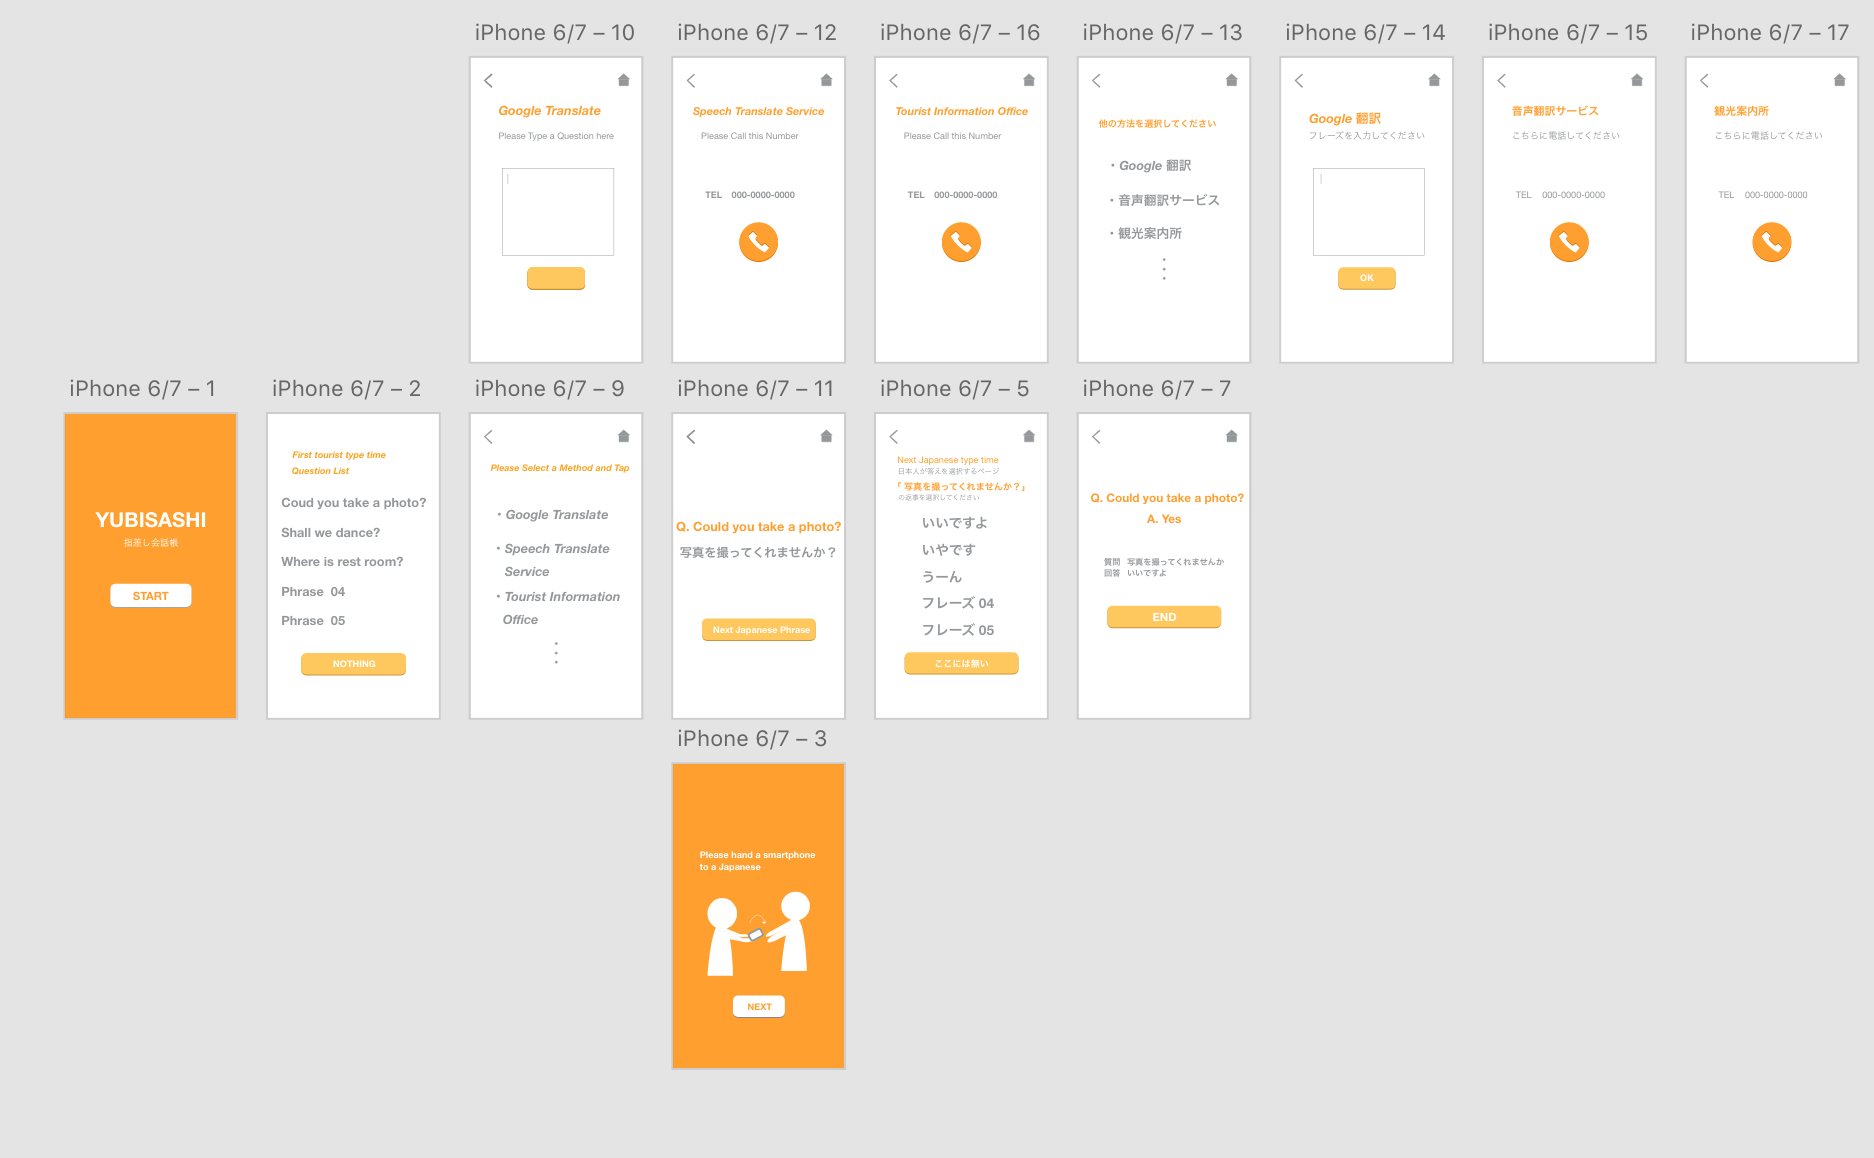
\includegraphics[width=20cm,angle=90]{moc.png}
\end{center}

%付録の終わり
\end{appendix}


%\backmatter

% 参考文献
\begin{thebibliography}{9}
 \bibitem{1}函館市観光部観光企画課 「来函観光入込客数推計」による。
  (http://www.city.hakodate.hokkaido.jp/docs/2015062500021/files/H28irikomi.pdf)
 %\bibitem {ラベル} 著者名. 書籍名. 出版社,  年号.
 %\bibitem {A2} ほげほげお. うんたらかんたら,  2003.
\end{thebibliography}

\end{document}
